\section{Study Design}
\label{sec:design}

\subsection{Overview}


\begin{figure*}[t]
    \centering
    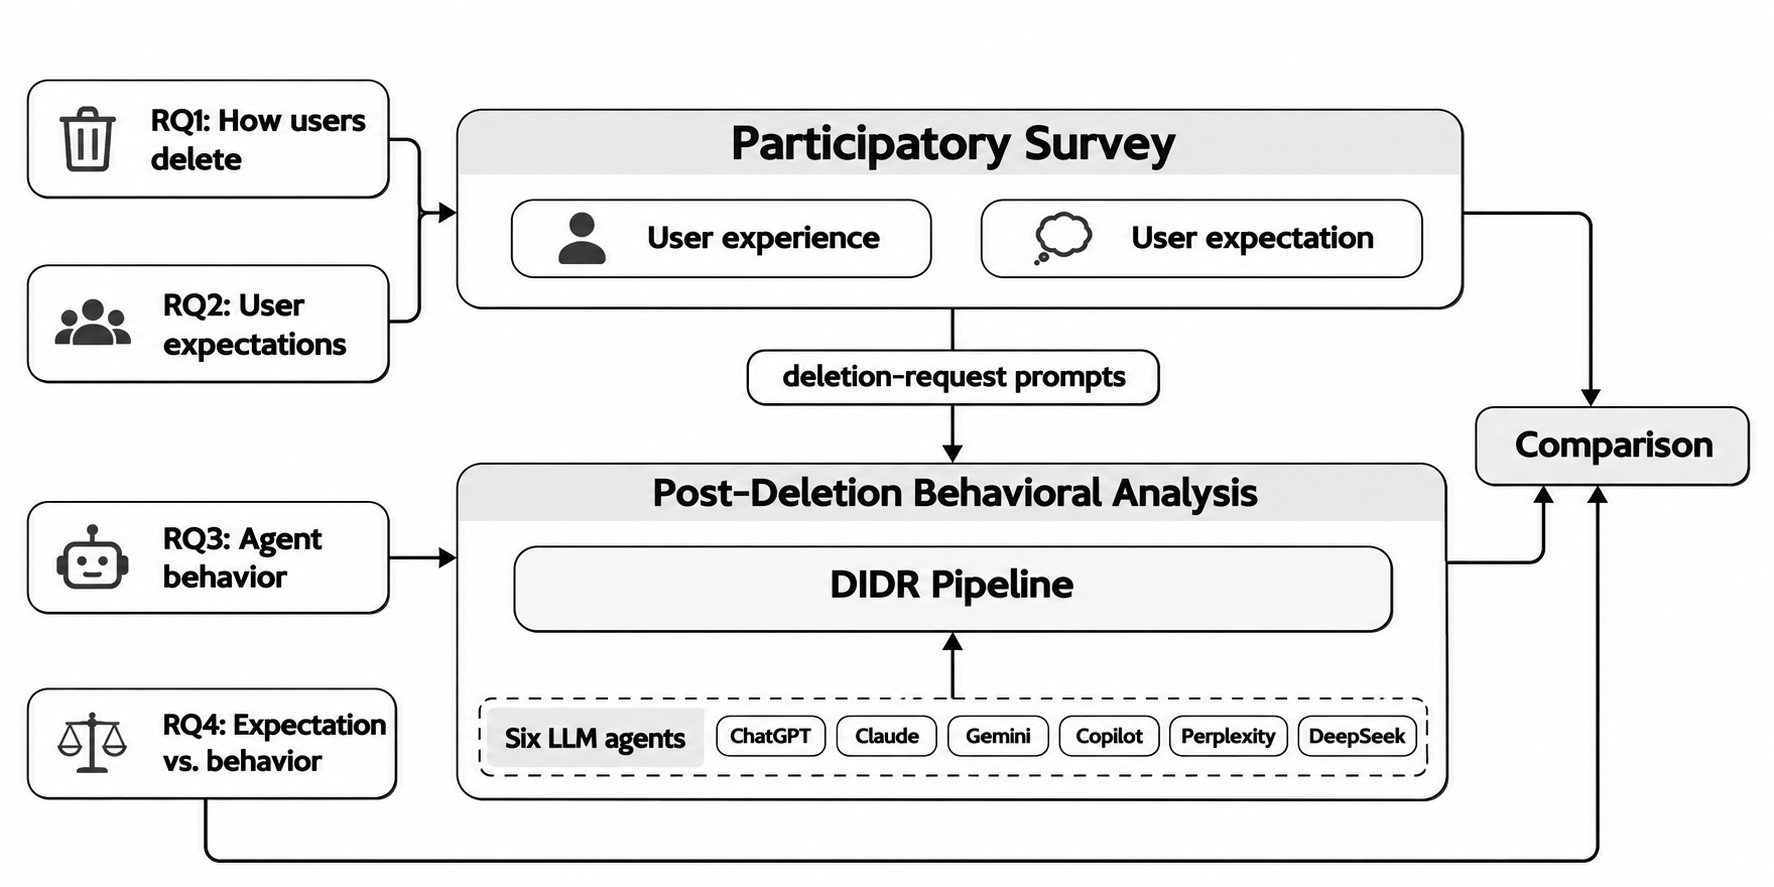
\includegraphics[width=0.9\textwidth]{figures/high-level.png}
    \caption{Overview of the study. The participatory survey answers RQ1 and RQ2, and its deletion requests feed the Post-Deletion Behavioral Analysis, which answers RQ3. Comparing the two answers RQ4.}
    \label{fig:overview}
\end{figure*}

We examine data deletion in commercial LLM agents from two complementary perspectives: users' expectations and agents' post-deletion behavior (Figure~\ref{fig:overview}). First, a participatory survey examines how users approach data deletion across two scenarios, including their choice of deletion method, deletion-request prompts, expectations, and verification strategies. We then use the collected deletion requests in a Post-Deletion Behavioral Analysis, where we inject synthetic facts into six commercial LLM agents, apply deletion methods, and subsequently probe for data recall. Finally, we compare survey responses with observed agent behavior to identify discrepancies between users' expectations and what deletion achieves in practice.


Our four research questions follow this design. The survey answers RQ1 (How do users delete data from LLM agents, and does scenario sensitivity change what they do?) and RQ2 (What do users expect deletion to do, and how do they check that it worked?). The post-deletion analysis answers RQ3 (What do agents do after a deletion request, and how do they differ from each other?). Only the two together answer RQ4 (Where do user expectations and agent behavior differ?).


\subsection{Participatory Survey}

\subsubsection{Participant recruitment}

We recruited U.S. adults through Prolific who had used at least one of the six LLM agents described in Section~\ref{sec:background}. The survey was administered through Qualtrics, with a recruitment target of approximately 200 participants rather than a power-based sample size. Participants received \$4 each.

Of 235 submissions, 17 were incomplete and one failed an attention check. We excluded another 36 respondents who reported no prior experience deleting data from an LLM agent, as the survey examined deletion practices and expectations among users with such experience. Of the remaining 181 participants, four did not complete the method-choice question in both scenarios, yielding a final survey sample of 177. Separately, deletion-request prompts for the Post-Deletion Behavioral Analysis were drawn from 209 participants, including those without prior deletion experience, because the request-writing task was hypothetical (Section~\ref{sec:didr}).

Among the 177 participants, 73.4\% were under 45, and 62.1\% held at least a bachelor's degree (Appendix~A). Our findings therefore characterize users with prior deletion experience rather than the broader population of LLM-agent users.

\subsubsection{Survey design}

To address RQ1 and RQ2, we designed a survey examining users' deletion practices, perceptions of deletion methods, expectations, and verification strategies. Participants evaluated two scenarios differing in data sensitivity. The less sensitive scenario involved sharing a city while requesting weather information, while the more sensitive scenario involved disclosing a home address when seeking a clinic for a sexually transmitted infection. In both scenarios, participants considered deleting the shared location data. The scenarios used identical questions and were presented in randomized order to mitigate order effects. We refer to the less sensitive scenario as \textbf{LS} and the more sensitive scenario as \textbf{MS}, and label analyses that combine both scenarios as \textbf{Pooled}. The survey used the term ``AI chatbot'' to refer to LLM agents.

Participants first indicated which of eight deletion methods they had previously used: the six listed in Table~\ref{tab:methods}, account deletion, and filing a deletion request. In each scenario, they selected a method from those previously used and rated its perceived protection, effort, and benefit loss using five-point agreement scales comprising five, four, and three items, respectively. They also selected a preferred method from all eight options, regardless of prior experience. Additional questions assessed willingness to delete, expected deletion outcomes, and verification practices. Participants then wrote the deletion request they would send to the agent.

Before the scenarios, participants reported which LLM agents they had used and their duration of use. Following the scenarios, they answered questions about prior deletion experiences, including the types of data they had attempted to delete, their motivations, and whether deleted information had resurfaced. The survey concluded with a privacy-knowledge quiz, questions about attitudes toward LLM agents and data sharing, and demographic questions. Two instructed-response items served as attention checks. Appendix~B provides the complete scenarios, measurement items, and attention checks.

\subsubsection{Data analysis}

We report percentages of the 177 participants, within LS or MS. Because every participant answered in both scenarios, we compared LS and MS within participants. We compared willingness to delete, protection, effort, and benefit loss with Wilcoxon signed-rank tests, and the data deletion method chosen overall with a Stuart-Maxwell test on the 176 participants who chose a data deletion method in both LS and MS. We compared each data deletion method, expectation option, and verification option between LS and MS with McNemar tests.

To compare data deletion methods, we used Pooled analyses, so each participant contributed two responses, and a response is one participant's answer in one scenario. We fitted generalized estimating equations clustered by participant so that the paired responses are not treated as independent. We included only the four data deletion methods chosen by at least 14 participants, because smaller groups give unstable estimates, which left 317 of the 354 responses after we dropped 2 Other responses and the 35 responses on the three data deletion methods below the minimum. The ratings used Gaussian models and the expectation options used logistic models, with scenario as a covariate, and we tested pairwise differences in effort between data deletion methods with GEE contrasts. We compared verification options by data deletion method with chi-square or Fisher's exact tests, separately in each scenario, because within one scenario each participant contributes a single response. A three-factor confirmatory factor analysis on the 354 responses, one factor each for protection, effort, and benefit loss, checked that the scales measure separate things (Appendix~C.2).

We treated the analyses as exploratory and applied the Holm correction within each family, the set of tests asking the same question across the three scales, seven data deletion methods, seven expectation options, eight verification options, or six pairs of data deletion methods. We report adjusted values as $p_{\mathrm{Holm}}$ and left single tests unadjusted. Table~\ref{tab:analysis-families} lists each analysis, its test, its base, and its family. The written deletion requests are coded and sampled in the post-deletion analysis (Section~\ref{sec:didr}), not here.

\subsection{Post-Deletion Behavioral Analysis}
\label{sec:didr}


To observe what agents do after a deletion request, we built a pipeline that injects a known fact into an agent, deletes it, and later tests whether the agent still returns it: the data injection, deletion, and recall (DIDR) pipeline (Figure~\ref{fig:didr}). Because we plant the fact ourselves, we know exactly what the agent was told, and a later recall can be traced back to it. Each test case combines one fact, one way of injecting and deleting it, and one agent. The pipeline starts with synthetic fact generation, which produces the facts we inject into commercial LLM agents. The pipeline runs in two parts. Through UI actions, we walk through each agent's interface and inject and delete facts in every way it offers, from typing in the chat to using memory pages and history controls. Through prompts, we inject a fact with a conversational disclosure and delete it with a deletion request that a participant wrote in the survey. In both parts, we delete at least 48 hours after injection, so the agent has time to process the fact, and we run data recall at least 30 days after deletion, so that the up to 30 days some agents document for deleted data have passed. Data recall tests whether the agent still returns the fact, through recall prompts and a UI-based check. Playwright-based automation drives the three stages where a control can be automated, and we ran the others by hand (for example Gemini's activity deletion, where we chose a time frame that held the injection).
    
\begin{figure*}[t]
    \centering
    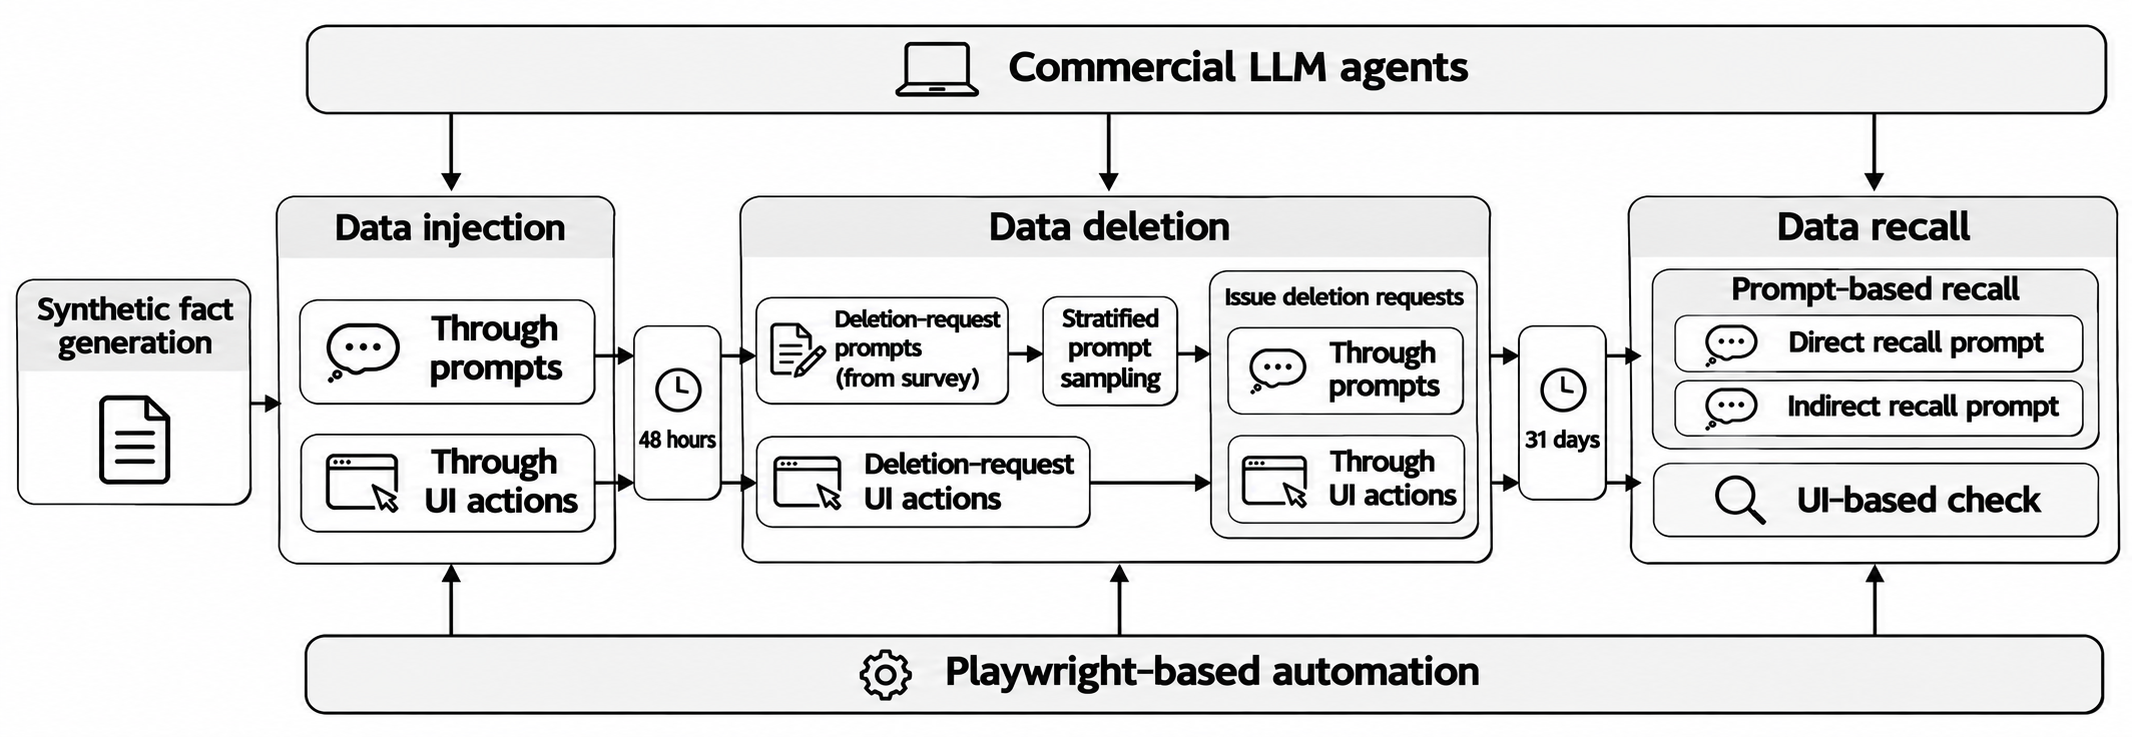
\includegraphics[width=\textwidth]{figures/DIDR.png}
    \caption{The DIDR pipeline. Synthetic facts are injected into commercial LLM agents, followed by deletion at least 48 hours later and recall testing at least 30 days after deletion. Each stage uses prompt-based and UI-based interactions, automated with Playwright.}
    \label{fig:didr}
\end{figure*}

\para{Synthetic fact generation}

To trace any later recall to the fact that caused it, each test case needs a fact the agent could not already know. We therefore generate synthetic facts, each a tuple of an entity, an attribute, and a value. The entity is an ordinary thing a person might mention in passing, such as a scarf being knitted or a sourdough starter. The attribute is its name. The value is a made-up code name of two to four words. For example, one fact is $\langle$a scarf I'm knitting, name, ``Magnifier King Broom''$\rangle$. Each value is unique to one test case, following the canary approach of Carlini et al.~\cite{carlini2019secret}, so a recall of the value identifies the test case it came from. We wrote the entities ourselves, from curated lists of everyday objects and projects. We drew each value from the EFF long word list, kept only words with a noun sense in WordNet, and removed words under WordNet's weapon, drug, and sexual-content categories, along with a short list of other terms, because content that a platform's safety filter might intercept would confuse a filtered answer with a deleted fact. Each fact is delivered in a casual sentence that varies across test cases, because a single repeated template would look unlike real chat.

\para{Data injection}

We inject each fact in the ways people put information into agents, and we use more than one because each reaches a different place where an agent may keep it. Through UI actions, we inject each fact in every way the agent's interface allows: mentioned in passing in a conversation, as an explicit request to remember it, or entered on a page such as a memory page, custom instructions, or Gemini's saved-info page. We found these by walking through each agent's web interface and listing every way a user can put information in, an approach similar to earlier walkthroughs of LLM privacy controls~\cite{li2026privacy}. Where an agent offers only some of these, we use those. Through prompts, every fact is a casual sentence mentioned in passing in a chat, always the same way in, so injection is held constant and only the deletion request varies. Deletion follows at least 48 hours after injection, which gives the agent time to process the fact, such as saving it to memory, before we delete it.

\para{Data deletion}

Through UI actions, we use the data deletion methods from the walkthrough (Table~\ref{tab:methods}). One of them, sending a deletion-request prompt, is typed in the chat, so 13 of the test cases through UI actions are typed requests. Each acts on a place where an agent may keep the fact, such as the conversation, saved memories, a saved-info page, activity history, or a privacy dashboard. For each agent we also ran the most extensive deletion, the combination of all its controls and the most a careful user could do, to see whether anything still comes back. We did not test two of the survey's eight methods: deleting the account, because nothing is left to observe, and filing a request with the company, because it is handled outside the agent. Test cases whose deletion could affect others, such as account-wide actions, ran on dedicated accounts, and deletions that share an account ran from narrowest to broadest, so that no deletion clears another test case's fact before its own recall. This gives 73 test cases through UI actions across the six agents, of which we could run 67, because six Perplexity controls need a paid plan.

Through prompts, we take the deletion requests from the survey so that they match how users actually ask. In total, 209 participants wrote 415 requests, including participants without deletion experience, because the task was hypothetical. After removing repeats and duplicates, 375 distinct requests remained, and we redacted identifying details from 7 of them. Testing all 375 on six agents would have meant 2,250 test cases under free-tier rate limits, so we tested a sample chosen to be representative and to avoid redundant tests. We grouped the requests into seven groups with keyword rules, for example whether a request mentions memory, the conversation, the account, or a database, and drew 138 requests by stratified random sampling, with at least 15 per group so the two smallest groups were included in full. The groups only spread the sample and are not used in any analysis. Two researchers then coded the 138 requests on seven dimensions of wording, such as where a request asks to delete and how politely it is phrased, so that we can test whether wording affects the outcome. They first coded a subset of 50 without a shared codebook, reconciled their candidate dimensions into one codebook, and refined it through further independent rounds on that subset. They then independently coded all 138 requests, and agreement was high (Gwet's AC1 of 0.954 pooled over the seven dimensions; Appendix~D). We settled disagreements through discussion and use the settled codes in all analyses. Five requests asked to delete all of a user's data and could have deleted other test cases' facts, so we excluded them. We sent the remaining 133 to all six agents after injecting a fact through a prompt, which gives 798 test cases. Together with the 67 test cases through UI actions, we ran 865 test cases. We also tested uploaded files as a separate group of 12 test cases, deleting the conversation and applying the most extensive deletion on each agent, because an agent can read an uploaded document, save it to memory, do both, or do neither. We report the 11 we could run one by one; the most extensive deletion on Perplexity needs a paid plan.

We also code the agents' replies to deletion requests submitted through chat. Two researchers independently classify each reply as \textit{complied}, \textit{partial}, \textit{deflected}, \textit{refused}, \textit{silently ignored}, or \textit{other} (Appendix~D), judging only what the agent said and not whether anything was deleted. Agreement is high (Gwet's AC1 = 0.969 across 788 replies), and we resolve disagreements through discussion. Deletions through UI actions have no reply to code.



\para{Data recall}

We conduct recall tests at least 30 days after deletion, because ChatGPT, Claude, and Perplexity document that deleted data can persist in their systems for up to 30 days. We apply the same minimum interval across all six agents for comparability. We assess recall with direct and indirect recall prompts in a new conversation, and with a UI-based check. Direct prompts explicitly ask about the entity and its attribute, while indirect prompts request an ordinary task involving the entity without mentioning the attribute or its value. This distinction allows us to examine both explicit retrieval and whether previously disclosed information surfaces without being requested. Each prompt type is issued twice with different wording, because replies vary between runs and a single wording could miss by chance. We check the replies for the injected value and manually review all of them.

The UI-based check examines the agent's memory or saved-information page, independently of its replies. It applies only where such a page is available and is therefore omitted for DeepSeek, Perplexity, and Copilot accounts without an accessible memory page. We perform the UI-based check first, followed by the indirect and direct recall prompts, so that an explicit recall prompt cannot influence the other checks. When deletion is requested in the original conversation, we also send the first direct prompt there and report it separately, since the disclosure is still in that conversation's context.

We classify a test case as \textit{recall success} if any applicable check returns the injected value. A case is classified as \textit{recall failed} only when no check retrieves the value and there is evidence that the fact was initially saved in the tested location; otherwise, the outcome is \textit{can't tell}. We establish evidence of initial storage from the replies and screenshots saved at injection. A fact is considered saved only when the interface displays an explicit memory notification, such as ``Memory updated'', or the agent explicitly states that it saved the information. Generic acknowledgments, such as ``Got it'', are insufficient. Ambiguous replies are resolved through manual review. We also count recall replies that withhold the fact because of an earlier deletion or non-use request, found by phrase matching and checked by hand; they do not change the recall outcome.

For deletions through UI actions, we also examine whether the relevant interface reflects the requested deletion, such as a conversation disappearing from history or a saved fact disappearing from memory. We assess these changes using post-deletion screenshots and inspect the account directly when the screenshots are inconclusive. Interface changes are not observable for deletion requests submitted through chat.

We additionally assess whether observed behavior is consistent with each agent's published documentation. For each test case, we classify the documented commitment according to the deletion method and injection location as \textit{deletes}, \textit{does not delete}, \textit{no commitment}, \textit{unrelated}, or \textit{not testable}. Only \textit{deletes} (the documentation says the method removes the content) and \textit{does not delete} (it says the method does not reach it) support consistency verdicts. For \textit{deletes}, recall success or an unchanged interface contradicts the commitment, while recall failed with a changed or unobservable interface is consistent with it. Recall success from past conversations alone is also consistent when the documentation says past conversations remain. For \textit{does not delete}, recall success is consistent. Cases with a \textit{can't tell} outcome remain unresolved, and the other commitment categories receive no consistency verdict.

Finally, we examine whether deletion-request wording is associated with recall outcomes by comparing recall-success counts across coding categories within each agent. Because some categories contain few requests, we report descriptive counts without statistical tests and restrict comparisons to categories containing at least six deletion requests. Agents whose test cases are all classified as \textit{can't tell} are excluded.

\para{Comparing expectations with behavior}
To find where expectations and behavior differ, we take each data deletion method that participants chose in the survey and look at the test cases that used the same method. The survey percentages are shares of participants' responses and the post-deletion percentages are shares of test cases, so we do not compare the two numbers directly. We ask instead whether what participants expected held up in the post-deletion analysis. We make two comparisons. We set what participants expected deletion to do against whether the fact came back, which is recall success, and we set the checks participants said they used, asking the agent in the same conversation and looking at whether the interface changed, against what those checks showed in our test cases.
